\chapter{Diagramas binários líquido--vapor e destilação}\label{ch:b2:liquid-vapour-diagrams}

Um alambique de cobre transforma um vinho de alguns por cento de álcool em
uma aguardente muitas vezes mais forte; uma coluna de refinaria separa o
petróleo bruto em suas frações, do gás ao óleo combustível pesado. Ambos se
baseiam em um único fato: o vapor sobre uma mistura em ebulição é mais rico
no componente mais volátil do que o líquido. Repita a evaporação e a
condensação um número suficiente de vezes e a separação fica tão nítida
quanto se queira --- com uma exceção: nenhuma destilação, por mais longa que
seja a coluna, leva o etanol além de cerca de 95 por cento em massa. Este
capítulo traça os diagramas que dizem como uma mistura de dois líquidos
ferve e os usa para projetar uma coluna e para ver onde ela precisa parar.

\begin{recall}
\Cref{ch:b2:chemical-potential}: o \omterm{def:b2:chemical-potential:chemical-potential}{potencial químico}, a \omterm{thm:b2:chemical-potential:raoult}{lei de Raoult} e a
\omterm{def:b2:chemical-potential:ideal-mixture}{mistura ideal}, os \omterm{def:b2:chemical-potential:activity-coefficient}{coeficientes de atividade} e os desvios em relação à \omterm{thm:b2:chemical-potential:raoult}{lei de
Raoult}, a relação de Gibbs--Duhem. \Cref{ch:b2:equilibrium-shifts}: a
\omterm{def:b2:equilibrium-shifts:variance}{variância}. O volume do 1.º ano, sobre as técnicas de laboratório: a
destilação simples, os líquidos miscíveis e imiscíveis. O volume escolar: a
destilação e a hidrodestilação.
\end{recall}

\begin{omfigure}
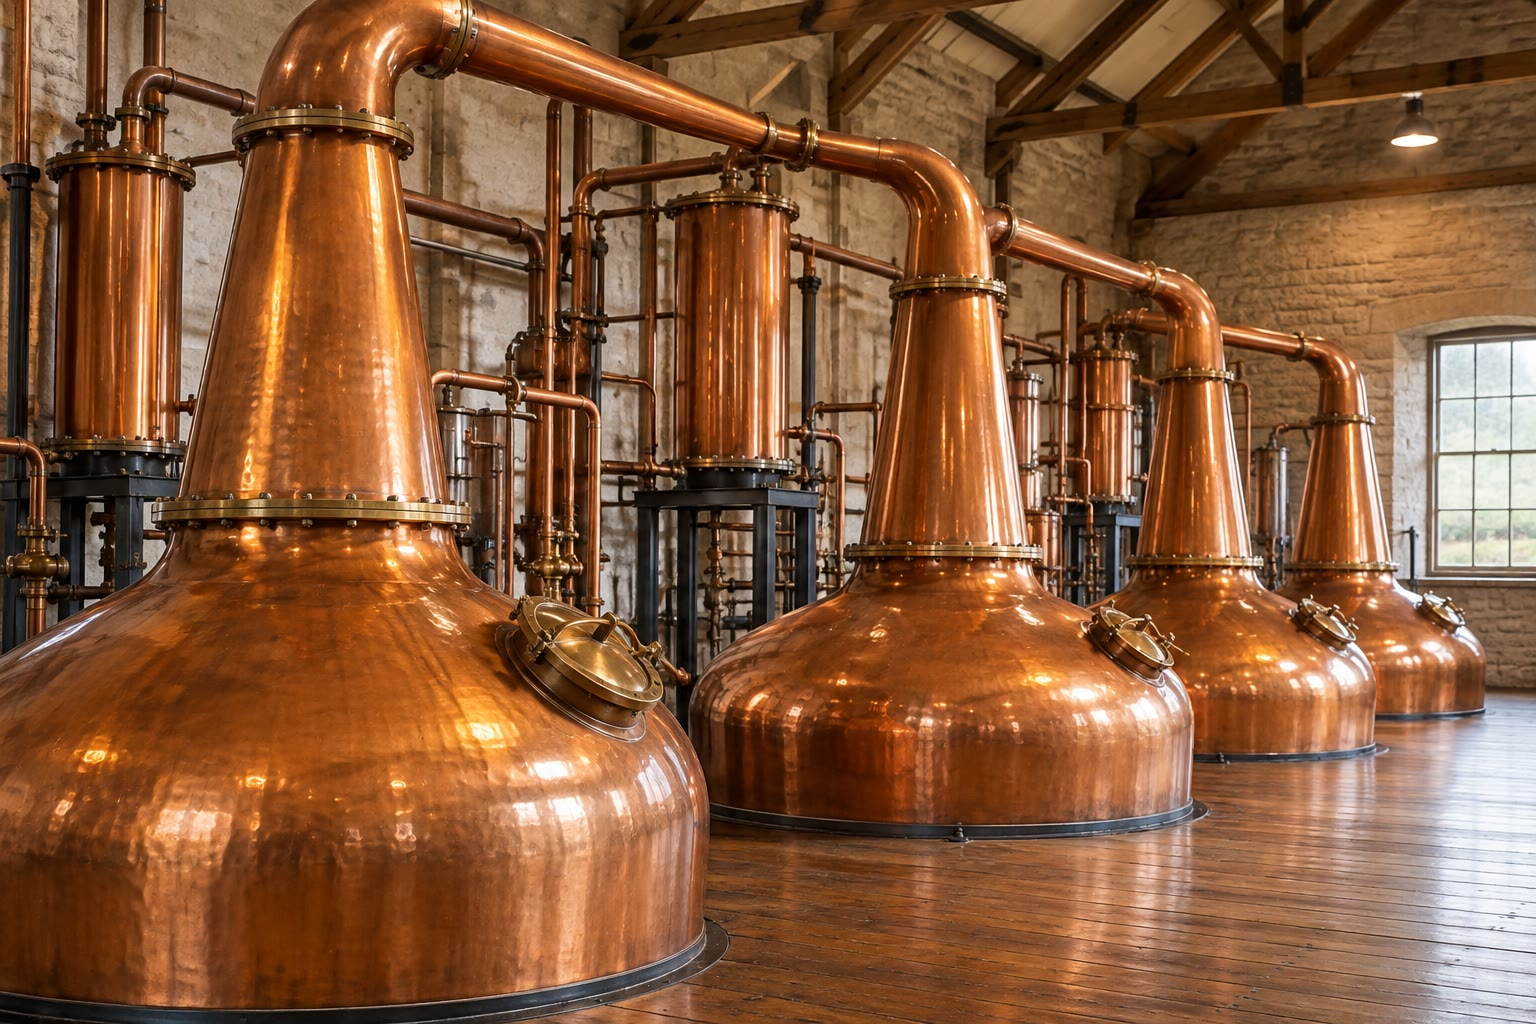
\includegraphics[width=0.62\linewidth]{images/book3/ai/b2-07-pot-stills.jpg}

{\small Alambiques de cobre em uma destilaria. Cada carga de mosto fermentado
é fervida e seu vapor, condensado: o primeiro destilado é várias vezes mais
rico em etanol que o mosto, e uma segunda destilação o concentra ainda mais.}
\end{omfigure}

\section{Misturas ideais}

Neste capítulo, os dois líquidos são numerados 1 (o mais volátil, de ponto
de ebulição mais baixo) e 2; $x$ é a fração molar de 1 no líquido, $y$ sua
fração molar no vapor, que é tratado como um gás ideal.

\begin{definition}[Diagrama binário]\label{def:b2:liquid-vapour-diagrams:binary-diagram}
Um \emph{diagrama binário}\index{diagrama binario@diagrama binário} mostra, para uma mistura de dois
componentes, quais fases estão presentes e com quais composições, em função
da composição global e de uma outra variável. Um
\emph{diagrama isobárico}\index{diagrama isobarico@diagrama isobárico} é traçado no plano
(composição, temperatura) a pressão fixa; um \emph{diagrama
isotérmico}\index{diagrama isotermico@diagrama isotérmico}, no plano (composição, pressão) a
temperatura fixa.
\end{definition}

\begin{definition}[Curvas de bolha e de orvalho]\label{def:b2:liquid-vapour-diagrams:bubble-dew}
Em um diagrama líquido--vapor, a \emph{curva de bolha}\index{curva de bolha} dá
a composição do líquido em equilíbrio com o vapor; a \emph{curva de
orvalho}\index{curva de orvalho}, a do vapor em equilíbrio com o líquido. Para uma
mistura de composição dada a pressão fixa, o \emph{ponto de
bolha}\index{ponto de bolha} é a temperatura na qual a primeira bolha de
vapor aparece no aquecimento; o \emph{ponto de orvalho}\index{ponto de orvalho}, a
temperatura na qual a primeira gota de líquido aparece ao resfriar o vapor.
\end{definition}

\begin{proposition}[Curvas ideais]\label{prop:b2:liquid-vapour-diagrams:ideal-curves}
Para uma \omterm{def:b2:chemical-potential:ideal-mixture}{mistura ideal} à temperatura $T$, sendo $p_1^*$ e $p_2^*$ as pressões
de vapor dos líquidos puros, a \omterm{def:b2:liquid-vapour-diagrams:bubble-dew}{curva de bolha} do \omterm{def:b2:liquid-vapour-diagrams:binary-diagram}{diagrama isotérmico} é a
reta $p = p_2^* + x(p_1^* - p_2^*)$, e a \omterm{def:b2:liquid-vapour-diagrams:bubble-dew}{curva de orvalho} é a
hipérbole
\[
  p = \frac{1}{y/p_1^* + (1 - y)/p_2^*} .
\]
\end{proposition}

\begin{proof}
A \omterm{thm:b2:chemical-potential:raoult}{lei de Raoult} dá as pressões parciais $p_1 = xp_1^*$ e $p_2 = (1 -
x)p_2^*$; sua soma é a pressão total, linear em $x$. No vapor,
$y = p_1/p$, logo $x = yp/p_1^*$ e $1 - x = (1 - y)p/p_2^*$; somando,
$1 = p\,[y/p_1^* + (1 - y)/p_2^*]$.
\end{proof}

\begin{proposition}[O vapor é mais rico no componente mais volátil]\label{prop:b2:liquid-vapour-diagrams:richer}
Para uma \omterm{def:b2:chemical-potential:ideal-mixture}{mistura ideal} com $p_1^* > p_2^*$ e $0 < x < 1$, $y > x$.
\end{proposition}

\begin{proof}
$y = xp_1^*/p$ com $p = xp_1^* + (1 - x)p_2^* < p_1^*$, pois $p$ é uma
média ponderada de $p_1^*$ e $p_2^*$, estritamente entre elas. Logo $y >
x$.
\end{proof}

O \omterm{def:b2:liquid-vapour-diagrams:binary-diagram}{diagrama isobárico} é o que descreve uma destilação, que ocorre à pressão
atmosférica. Ele não tem fórmula simples: para cada temperatura entre os
dois pontos de ebulição, calculam-se $p_1^*(T)$ e $p_2^*(T)$ (aqui com a
equação de Antoine, $\log_{10}(p^*/\unit{bar}) = A - B/(T + C)$, ajustada a
pressões de vapor medidas) e depois as composições do líquido e do vapor que
dão uma pressão total de \qty{1.013}{bar}:
\[
  x = \frac{p - p_2^*(T)}{p_1^*(T) - p_2^*(T)}, \qquad y = \frac{x\,p_1^*(T)}{p} .
\]
A \omterm{def:b2:liquid-vapour-diagrams:bubble-dew}{curva de bolha} deixa de ser uma reta; a \omterm{def:b2:liquid-vapour-diagrams:bubble-dew}{curva de orvalho} continua acima
dela, e o vapor, mais rico no componente leve.

\begin{example}[Benzeno e tolueno a \qty{90}{\degreeCelsius}]\label{ex:b2:liquid-vapour-diagrams:benzene-toluene}
O benzeno e o tolueno formam uma mistura quase ideal. A \qty{90}{\degreeCelsius},
as equações de Antoine dão $p_1^* = \qty{1.361}{bar}$ (benzeno) e $p_2^* =
\qty{0.542}{bar}$ (tolueno). A \qty{1.013}{bar}: $x = (1.013 - 0.542)/(1.361 -
0.542) = 0.575$ e $y = 0.575 \times 1.361/1.013 = 0.773$. Um líquido com 57.5~\%
de benzeno (em mols) ferve a \qty{90}{\degreeCelsius} e dá um vapor com
77~\%.
% ledger: antoine:benzene.A, antoine:benzene.B, antoine:benzene.C, antoine:toluene.A, antoine:toluene.B, antoine:toluene.C
\end{example}

\begin{omfigure}
\begin{tikzpicture}
\begin{axis}[omphase, width=0.47\linewidth, height=6cm, ymin=78, ymax=113,
  xlabel={$x$, $y$ (benzeno)}, ylabel={$T$ (\unit{\degreeCelsius})},
  title={\small isobárico, \qty{1.013}{bar}}]
\addplot[omliquidus] table[x=x, y=T] {figdata/out/bachelor-2-liquid-vapour-a.dat};
\addplot[omsolidus] table[x=y, y=T] {figdata/out/bachelor-2-liquid-vapour-a.dat};
\draw[tieline] (axis cs:0.405,95) -- (axis cs:0.626,95);
\fill (axis cs:0.5,95) circle (1.3pt);
\draw[->, thick] (axis cs:0.5,82) -- (axis cs:0.5,104) node[above, font=\scriptsize] {aquecimento};
\node[font=\scriptsize] at (axis cs:0.2,85) {líquido};
\node[font=\scriptsize] at (axis cs:0.85,108) {vapor};
\node[font=\scriptsize, omDef, anchor=north] at (axis cs:0.22,96) {bolha};
\node[font=\scriptsize, omThm, anchor=south west] at (axis cs:0.62,101) {orvalho};
\end{axis}
\end{tikzpicture}\hfill
\begin{tikzpicture}
\begin{axis}[omphase, width=0.47\linewidth, height=6cm, ymin=0.3, ymax=1.1,
  xlabel={$x$, $y$ (benzeno)}, ylabel={$p$ (\unit{bar})},
  title={\small isotérmico, \qty{80}{\degreeCelsius}}]
\addplot[omliquidus] table[x=x, y=pbub] {figdata/out/bachelor-2-liquid-vapour-b.dat};
\addplot[omsolidus] table[x=x, y=pdew] {figdata/out/bachelor-2-liquid-vapour-b.dat};
\node[font=\scriptsize] at (axis cs:0.75,0.98) {líquido};
\node[font=\scriptsize] at (axis cs:0.2,0.36) {vapor};
\end{axis}
\end{tikzpicture}

{\small Benzeno--tolueno, calculado pela \omterm{thm:b2:chemical-potential:raoult}{lei de Raoult} e pelas equações de
Antoine. À esquerda, à pressão atmosférica: \omterm{def:b2:liquid-vapour-diagrams:bubble-dew}{curva de bolha} (em azul) e \omterm{def:b2:liquid-vapour-diagrams:bubble-dew}{curva
de orvalho} (em vermelho); o líquido de composição 0.5 começa a ferver a
\qty{92.1}{\degreeCelsius} e está todo vaporizado a \qty{98.8}{\degreeCelsius}; a
\qty{95}{\degreeCelsius} (linha de amarração tracejada), ele se divide em um
líquido de 0.405 e um vapor de 0.626. À direita, a \qty{80}{\degreeCelsius}: a
\omterm{def:b2:liquid-vapour-diagrams:bubble-dew}{curva de bolha} é uma reta, a \omterm{def:b2:liquid-vapour-diagrams:bubble-dew}{curva de orvalho} uma hipérbole, e o líquido
agora fica em cima.}
% ledger: antoine:benzene.A, antoine:toluene.A (all six parameters in figdata/bachelor-2/liquid-vapour.py)
\end{omfigure}

\section{Ler um diagrama}

\begin{proposition}[Variância de um binário bifásico]\label{prop:b2:liquid-vapour-diagrams:variance}
Uma mistura de dois componentes em duas fases tem \omterm{def:b2:equilibrium-shifts:variance}{variância} 2. A pressão fixa,
só a temperatura fixa as composições das duas fases: elas são lidas nas
extremidades do segmento horizontal que passa pelo ponto representativo,
chamado linha de amarração.
\end{proposition}

\begin{proof}
Variáveis intensivas: $T$, $p$, $x$, $y$. Relações: igualdade dos \omterm{def:b2:chemical-potential:chemical-potential}{potenciais
químicos} de 1 e de 2 entre as fases. $v = 4 - 2 = 2$ (a regra das fases
$v = n - r + 2 - \varphi$ dá o mesmo com $n = 2$, $r = 0$, $\varphi = 2$).
Fixar $p$ deixa um grau de liberdade: $x(T)$ e $y(T)$ são as duas curvas.
\end{proof}

\begin{theorem}[Regra da alavanca]\label{thm:b2:liquid-vapour-diagrams:lever}
Uma mistura de composição global $z$, dividida em um líquido de composição $x$
e um vapor de composição $y$, contém as quantidades $n_L$ de líquido e $n_V$ de
vapor tais que
\[
  n_L\,(z - x) = n_V\,(y - z), \qquad \frac{n_V}{n_L + n_V} = \frac{z - x}{y - x} .
\]
Essa é a \emph{regra da alavanca}\index{regra da alavanca}: cada fase é tanto mais
abundante quanto mais sua composição se aproxima da composição global, como os
pesos em uma alavanca apoiada em $z$.
\end{theorem}

\begin{proof}
Conservação do componente 1: $(n_L + n_V)z = n_Lx + n_Vy$, logo $n_L(z - x) =
n_V(y - z)$; divida por $n_L + n_V$ e rearranje.
\end{proof}

A \omterm{thm:b2:liquid-vapour-diagrams:lever}{regra da alavanca} vale com frações molares e quantidades de matéria, como
aqui, ou com frações mássicas e massas: a conservação usada é a mesma.

\begin{method}[Ler um diagrama binário]\label{met:b2:liquid-vapour-diagrams:read-diagram}
\begin{enumerate}
  \item Marque o ponto (composição global, temperatura) e identifique seu
        domínio: líquido, vapor ou líquido + vapor.
  \item Em um domínio bifásico, trace a linha de amarração pelo ponto; suas
        extremidades dão as composições do líquido (na \omterm{def:b2:liquid-vapour-diagrams:bubble-dew}{curva de bolha}) e do
        vapor (na \omterm{def:b2:liquid-vapour-diagrams:bubble-dew}{curva de orvalho}).
  \item Obtenha as proporções das fases pela \omterm{thm:b2:liquid-vapour-diagrams:lever}{regra da alavanca}.
  \item Para acompanhar um aquecimento, desloque o ponto para cima: a primeira
        bolha aparece na \omterm{def:b2:liquid-vapour-diagrams:bubble-dew}{curva de bolha}, a última gota desaparece na \omterm{def:b2:liquid-vapour-diagrams:bubble-dew}{curva de
        orvalho}; entre elas, o líquido fica cada vez mais pobre no componente leve.
\end{enumerate}
\end{method}

\begin{example}[Um flash a \qty{95}{\degreeCelsius}]\label{ex:b2:liquid-vapour-diagrams:flash}
\qty{100}{mol} de uma mistura equimolar de benzeno--tolueno são levados a
\qty{95}{\degreeCelsius} à pressão atmosférica. A linha de amarração dá $x =
0.405$, $y = 0.626$; a fração vaporizada é $(0.500 - 0.405)/(0.626 - 0.405) =
0.43$: \qty{43}{mol} de vapor contendo $43 \times 0.626 = \qty{27}{mol}$ de
benzeno, \qty{57}{mol} de líquido contendo \qty{23}{mol}. Um estágio de
equilíbrio enriquece, mas só um pouco.
\end{example}

\section{Misturas reais e azeótropos}

Quando os \omterm{def:b2:chemical-potential:activity-coefficient}{coeficientes de atividade} diferem de 1 (\cref{ch:b2:chemical-potential}),
as pressões parciais se afastam das retas de Raoult. Com um desvio positivo
($\gamma > 1$: moléculas diferentes se atraem menos que moléculas iguais), a
pressão total fica acima da reta ideal; com um desvio negativo, abaixo. Se o
desvio for forte o bastante, a pressão total passa por um extremo.

\begin{definition}[Azeótropo]\label{def:b2:liquid-vapour-diagrams:azeotrope}
Um \emph{azeótropo}\index{azeotropo@azeótropo} é uma mistura líquida que ferve sem
mudar de composição: o vapor que ela dá tem a mesma composição que ela. Um
\emph{azeótropo positivo}\index{azeotropo positivo@azeótropo positivo} (desvio positivo) tem
um máximo de pressão no \omterm{def:b2:liquid-vapour-diagrams:binary-diagram}{diagrama isotérmico} e um mínimo de temperatura de
ebulição no isobárico; um \emph{azeótropo negativo}\index{azeotropo negativo@azeótropo negativo},
o inverso.
\end{definition}

\begin{theorem}[Gibbs--Konovalov]\label{thm:b2:liquid-vapour-diagrams:konovalov}
Em um \omterm{def:b2:liquid-vapour-diagrams:binary-diagram}{diagrama binário} líquido--vapor, em um extremo da pressão total (a
temperatura fixa) ou da temperatura de ebulição (a pressão fixa), o líquido
e o vapor têm a mesma composição. Reciprocamente, onde as duas composições
são iguais, as curvas têm uma tangente horizontal comum.
\end{theorem}

\begin{proof}[Demonstração a temperatura fixa]
A relação de Gibbs--Duhem para o líquido a $T$ fixo (desprezado o pequeno
efeito de $p$ sobre o líquido) é $x\,d\mu_1 + (1 - x)\,d\mu_2 = 0$. No equilíbrio,
$\mu_i = \mu_i^\circ + RT\ln(p_i/p^\circ)$ com $p_1 = yp$, $p_2 = (1 - y)p$, logo
\[
  x\,d\ln(yp) + (1 - x)\,d\ln((1 - y)p) = 0
  \quad\Longrightarrow\quad
  d\ln p = -\Big(\frac{x}{y} - \frac{1 - x}{1 - y}\Big)dy
  = \frac{y - x}{y(1 - y)}\,dy .
\]
Como $y$ cresce com $x$ (senão o líquido seria instável),
$dp/dx = 0$ exatamente onde $y = x$. O caso isobárico decorre de um cálculo
semelhante, que conserva a dependência dos $\mu_i^\circ$ com a temperatura;
ele não é feito aqui.
\end{proof}

A fórmula diz mais: onde $y > x$, a pressão cresce com $x$ ---
adicionar o componente que se enriquece no vapor torna o líquido mais
volátil, o que é a primeira lei de Konovalov.

\begin{example}[Etanol e água]\label{ex:b2:liquid-vapour-diagrams:ethanol-water}
O etanol e a água apresentam um desvio positivo em relação à \omterm{thm:b2:chemical-potential:raoult}{lei de Raoult} e
formam um \omterm{def:b2:liquid-vapour-diagrams:azeotrope}{azeótropo} com 95~\% de etanol em massa à pressão atmosférica. Com
$M = 46.07$ e \qty{18.02}{g/mol}, sua fração molar de etanol é
\[
  x_{\text{az}} = \frac{95/46.07}{95/46.07 + 5/18.02} = 0.881 .
\]
Ele ferve um pouco abaixo do etanol puro (\qty{78.3}{\degreeCelsius}). O
diagrama abaixo é calculado com um modelo de atividade de um parâmetro, $\ln\gamma_1 = A(1 -
x)^2$, $\ln\gamma_2 = Ax^2$, cujo parâmetro ($A = 1.09$) é ajustado para que o
\omterm{def:b2:liquid-vapour-diagrams:azeotrope}{azeótropo} caia nessa composição: o modelo reproduz a forma e situa o
\omterm{def:b2:liquid-vapour-diagrams:azeotrope}{azeótropo} a \qty{77.9}{\degreeCelsius}.
% ledger: azeo:ethanol-water.w, aw:C, aw:H, aw:O, antoine:ethanol.A, antoine:ethanol.B, antoine:ethanol.C, antoine:water.A, antoine:water.B, antoine:water.C
\end{example}

\begin{omfigure}
\begin{tikzpicture}
\begin{axis}[omphase, width=0.47\linewidth, height=6cm, ymin=76, ymax=101,
  xlabel={$x$, $y$ (etanol)}, ylabel={$T$ (\unit{\degreeCelsius})},
  title={\small etanol--água (modelo)}]
\addplot[omliquidus] table[x=x, y=T] {figdata/out/bachelor-2-liquid-vapour-c.dat};
\addplot[omsolidus] table[x=y, y=T] {figdata/out/bachelor-2-liquid-vapour-c.dat};
\fill (axis cs:0.881,77.92) circle (1.5pt);
\draw[densely dotted] (axis cs:0.881,77.92) -- (axis cs:0.881,76);
\node[font=\scriptsize, anchor=south] at (axis cs:0.80,80.5) {azeótropo};
\draw[thin] (axis cs:0.80,80.5) -- (axis cs:0.875,78.2);
\node[font=\scriptsize] at (axis cs:0.25,79.5) {líquido};
\node[font=\scriptsize] at (axis cs:0.5,95) {vapor};
\end{axis}
\end{tikzpicture}\hfill
\begin{tikzpicture}
\begin{axis}[omphase, width=0.47\linewidth, height=6cm, ymin=78, ymax=120,
  xlabel={$x$, $y$ (componente 1)}, ylabel={$T$ (\unit{\degreeCelsius})},
  title={\small desvio negativo (modelo)}]
\addplot[omliquidus] table[x=x, y=T] {figdata/out/bachelor-2-liquid-vapour-d.dat};
\addplot[omsolidus] table[x=y, y=T] {figdata/out/bachelor-2-liquid-vapour-d.dat};
\fill (axis cs:0.29,116.7) circle (1.5pt);
\node[font=\scriptsize, anchor=west] at (axis cs:0.33,118) {azeótropo};
\node[font=\scriptsize] at (axis cs:0.6,85) {líquido};
\node[font=\scriptsize] at (axis cs:0.75,116) {vapor};
\end{axis}
\end{tikzpicture}

{\small À esquerda: etanol--água à pressão atmosférica, com um modelo de um
parâmetro ajustado à composição do \omterm{def:b2:liquid-vapour-diagrams:azeotrope}{azeótropo} (0.881); o \omterm{def:b2:liquid-vapour-diagrams:azeotrope}{azeótropo} ferve
abaixo dos dois líquidos puros. À direita: um par modelo com um forte desvio
negativo ($A = -2.0$, pressões de vapor do benzeno e do tolueno); o
\omterm{def:b2:liquid-vapour-diagrams:azeotrope}{azeótropo} ferve acima dos dois.}
% ledger: azeo:ethanol-water.w, antoine:ethanol.A, antoine:water.A (model in figdata/bachelor-2/liquid-vapour.py)
\end{omfigure}

\section{Destilação fracionada}

\begin{definition}[Destilação fracionada]\label{def:b2:liquid-vapour-diagrams:fractional-distillation}
A \emph{destilação fracionada}\index{destilacao fracionada@destilação fracionada} separa os
componentes de uma mistura líquida em uma coluna na qual um vapor ascendente
e um líquido descendente são postos em contato repetidamente. Um \emph{prato
teórico}\index{prato teorico@prato teórico} é um estágio da coluna cujos vapor e líquido de saída
estão em equilíbrio entre si. A \emph{razão de
refluxo}\index{razao de refluxo@razão de refluxo} é a razão entre a quantidade de condensado
devolvida ao topo da coluna e a quantidade retirada como destilado.
\end{definition}

Em cada prato, o vapor vindo de baixo borbulha através do líquido vindo de
cima; ele sai mais rico no componente leve, e o líquido, mais pobre. No topo,
o vapor é condensado, parte dele é devolvida como refluxo e o resto é retirado
como destilado; na base, um refervedor ferve parte do líquido. Em
\textit{refluxo total}, nada é retirado: a coluna funciona então em seu
melhor desempenho, e o vapor que sai de um prato tem a composição do líquido
que desce sobre ele.


Para um par ideal, a \textit{volatilidade relativa} $\alpha = p_1^*/p_2^*$
varia pouco ao longo da coluna: de 2.60 no ponto de ebulição do benzeno a
2.35 no do tolueno. Em cada \omterm{def:b2:liquid-vapour-diagrams:fractional-distillation}{prato teórico},
\[
  \frac{y}{1 - y} = \frac{xp_1^*}{(1 - x)p_2^*} = \alpha\,\frac{x}{1 - x} .
\]

\begin{omfigure}
\begin{minipage}[b]{0.58\linewidth}\centering
\begin{tikzpicture}[font=\small, >={Stealth}, scale=0.8, every node/.style={transform shape}]
  \draw[thick, fill=gray!8] (0,0) rectangle (1.8,7);
  \foreach \k in {1,...,6} {
    \pgfmathsetmacro{\yy}{\k}
    \ifodd\k
      \draw[thick] (0,\yy) -- (1.45,\yy); \draw[thick] (1.45,\yy) -- (1.45,\yy-0.55);
    \else
      \draw[thick] (0.35,\yy) -- (1.8,\yy); \draw[thick] (0.35,\yy) -- (0.35,\yy-0.55);
    \fi
    \fill[omDef!25] (0.02,\yy) rectangle (1.78,\yy+0.12);
  }
  \foreach \k in {1,...,6} \node[font=\scriptsize, anchor=east] at (-0.1,\k) {prato \k};
  \draw[->, thick, omThm] (0.9,7.0) -- (0.9,7.9) -- (2.8,7.9);
  \draw[thick, fill=white] (2.8,7.6) rectangle (3.6,8.2);
  \node[anchor=west, font=\scriptsize] at (3.65,7.9) {condensador};
  \draw[->, thick, omDef] (3.2,7.6) -- (3.2,5.6);
  \draw[thick, fill=omDef!20] (2.7,5.0) rectangle (3.7,5.6);
  \node[font=\scriptsize, anchor=west] at (3.75,5.3) {tambor de refluxo};
  \draw[->, thick, omDef] (2.7,5.3) -- (2.1,5.3) -- (2.1,6.6) -- (1.8,6.6);
  \node[font=\scriptsize, anchor=west, omDef] at (2.15,6.1) {refluxo};
  \draw[->, thick, omDef] (3.2,5.0) -- (3.2,4.4) -- (4.4,4.4) node[right] {destilado};
  \draw[->, thick] (-2.2,3.5) -- (0,3.5) node[pos=0, left] {alimentação};
  \draw[thick, fill=omDef!20] (0.2,-1.3) rectangle (1.6,-0.6);
  \node[font=\scriptsize] at (0.9,-0.95) {refervedor};
  \draw[thick, omDef] (0.9,0) -- (0.9,-0.6);
  \draw[->, thick, omThm] (1.6,-0.8) -- (2.1,-0.8) -- (2.1,0.4) -- (1.8,0.4);
  \draw[->, thick, omDef] (0.9,-1.3) -- (0.9,-1.8) -- (2.6,-1.8) node[right] {produto de fundo};
  \draw[->, omThm, thick] (2.6,1.5) -- (2.6,3.0) node[midway, right, font=\scriptsize, align=left] {o vapor\\ sobe};
  \draw[->, omDef, thick] (-1.4,5.8) -- (-1.4,4.3) node[midway, left, font=\scriptsize, align=right] {o líquido\\ desce};
\end{tikzpicture}
\end{minipage}\hfill
\begin{minipage}[b]{0.34\linewidth}\centering
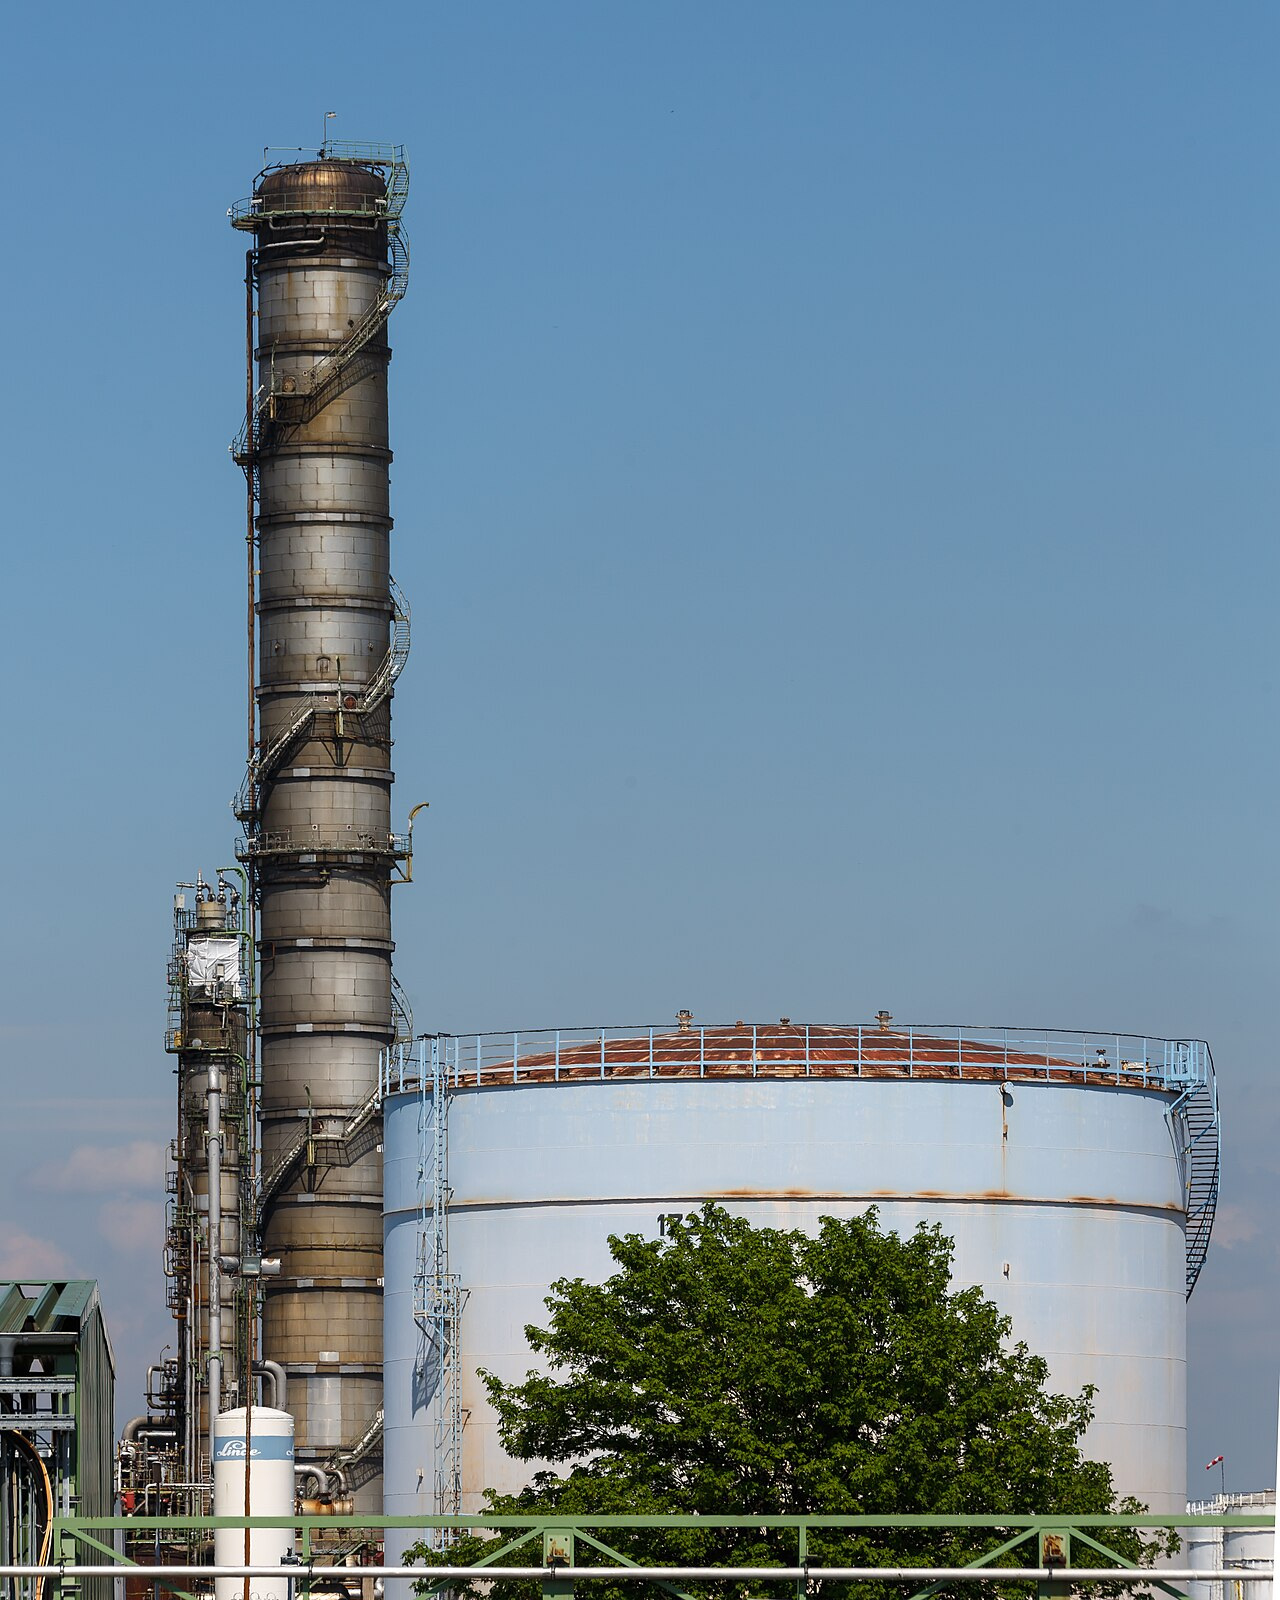
\includegraphics[width=\linewidth]{images/book3/refinery-column.jpg}
\end{minipage}

{\small À esquerda: uma coluna de pratos. O líquido escoa sobre cada prato e
desce pelo vertedor até o prato de baixo; o vapor sobe através dos pratos e
borbulha no líquido. O vapor condensado é em parte devolvido como refluxo; o
refervedor na base fornece o vapor. À direita: uma coluna de destilação de
uma refinaria (Colônia, 2014), que contém dezenas de pratos. (Fotografia:
CEphoto, Uwe Aranas, CC BY-SA 3.0, Wikimedia Commons.)}
\end{omfigure}

\begin{proposition}[Fenske]\label{prop:b2:liquid-vapour-diagrams:fenske}
A refluxo total, com uma volatilidade relativa $\alpha$ constante, o número de
\omterm{def:b2:liquid-vapour-diagrams:fractional-distillation}{pratos teóricos} necessário para ir de um líquido de fundo $x_B$ a um destilado
$x_D$ é no mínimo
\[
  N_{\min} = \frac{1}{\ln\alpha}\,\ln\!\left[\frac{x_D}{1 - x_D}\cdot\frac{1 - x_B}{x_B}\right] .
\]
\end{proposition}

\begin{proof}
Numere os pratos a partir de baixo, sendo o refervedor o prato 1. A refluxo total,
o líquido que desce sobre o prato $k + 1$ tem a composição do vapor que
sai do prato $k$: $x_{k+1} = y_k$. Com $r = x/(1 - x)$, cada prato dá
$r(y_k) = \alpha\,r(x_k)$, logo $r(x_{k+1}) = \alpha\,r(x_k)$ e, após $N$
pratos, o vapor condensado tem $r(x_D) = \alpha^N r(x_B)$. Tomando os
logaritmos, obtém-se $N$. Com um refluxo finito, o líquido que desce é mais
pobre que o vapor que sobe, cada prato enriquece menos, e são necessários
mais pratos.
\end{proof}

No diagrama $(x, y)$, a mesma construção é uma escada entre a curva de
equilíbrio e a diagonal $y = x$: cada degrau é um \omterm{def:b2:liquid-vapour-diagrams:fractional-distillation}{prato teórico}.

\begin{omfigure}
\begin{tikzpicture}
\begin{axis}[width=0.55\linewidth, height=0.55\linewidth, xmin=0, xmax=1,
  ymin=0, ymax=1, axis x line=bottom, axis y line=left,
  xlabel={$x$ (benzeno, líquido)}, ylabel={$y$ (benzeno, vapor)},
  tick label style={font=\small}, label style={font=\small}]
\addplot[omThm, thick] table[x=x, y=y] {figdata/out/bachelor-2-liquid-vapour-f-eq.dat};
\addplot[black!50] coordinates {(0,0) (1,1)};
\addplot[omDef, thick] table[x=x, y=y] {figdata/out/bachelor-2-liquid-vapour-f.dat};
\draw[densely dotted] (axis cs:0.95,0) -- (axis cs:0.95,0.95);
\draw[densely dotted] (axis cs:0.05,0) -- (axis cs:0.05,0.05);
\node[font=\scriptsize, anchor=south east] at (axis cs:0.945,0.02) {$x_D$};
\node[font=\scriptsize, anchor=south west] at (axis cs:0.05,0.02) {$x_B$};
\end{axis}
\end{tikzpicture}

{\small Pratos a refluxo total para benzeno--tolueno, a partir de um destilado
de 0.95: cada degrau horizontal vai de um vapor ao líquido em equilíbrio com
ele (um prato), cada degrau vertical, desse líquido ao vapor do prato de
baixo. Sete degraus levam o líquido abaixo de $x_B = 0.05$; a fórmula de
Fenske dá 6.5.}
% ledger: antoine:benzene.A, antoine:toluene.A (computed in figdata/bachelor-2/liquid-vapour.py)
\end{omfigure}

\begin{proposition}[Uma coluna não atravessa um azeótropo]\label{prop:b2:liquid-vapour-diagrams:azeotrope-limit}
Em uma mistura com um \omterm{def:b2:liquid-vapour-diagrams:azeotrope}{azeótropo}, uma coluna alimentada de um lado da
composição azeotrópica fornece, no melhor dos casos, o \omterm{def:b2:liquid-vapour-diagrams:azeotrope}{azeótropo} em uma
extremidade e o componente puro desse lado na outra.
\end{proposition}

\begin{proof}
No \omterm{def:b2:liquid-vapour-diagrams:azeotrope}{azeótropo}, a curva de equilíbrio encontra a diagonal: $y = x$. Perto dele,
cada degrau da escada se torna infinitamente pequeno; logo nenhum número
finito de pratos o atinge, e nenhum o atravessa.
\end{proof}

\begin{method}[Prever uma destilação fracionada]\label{met:b2:liquid-vapour-diagrams:predict-distillation}
\begin{enumerate}
  \item Encontre, no \omterm{def:b2:liquid-vapour-diagrams:binary-diagram}{diagrama isobárico}, o ponto de ebulição mais baixo
        acessível a partir da alimentação: um componente puro ou um \omterm{def:b2:liquid-vapour-diagrams:azeotrope}{azeótropo
        positivo}. Ele sai no topo.
  \item O ponto de ebulição mais alto do mesmo lado (componente puro ou
        \omterm{def:b2:liquid-vapour-diagrams:azeotrope}{azeótropo negativo}) fica no refervedor.
  \item Com um \omterm{def:b2:liquid-vapour-diagrams:azeotrope}{azeótropo}, veja de que lado dele está a alimentação: só o
        componente puro desse lado pode ser obtido.
  \item Para o número de pratos, use a fórmula de Fenske ou a escada e
        depois acrescente pratos para o refluxo finito realmente usado.
\end{enumerate}
\end{method}

Para etanol e água alimentados com menos de 0.881, o topo fornece, no melhor
dos casos, o \omterm{def:b2:liquid-vapour-diagrams:azeotrope}{azeótropo}, e o fundo, a água: nenhuma coluna dá etanol absoluto.
Secar o último por cento exige outro método --- uma peneira molecular que
adsorve a água, ou um terceiro componente adicionado para quebrar o \omterm{def:b2:liquid-vapour-diagrams:azeotrope}{azeótropo}.

\begin{omfigure}
\begin{tikzpicture}[font=\small, scale=0.95, >={Stealth}]
  \pic[transform shape] at (0,0) {heatingmantle};
  \pic[transform shape] at (0,0) {rbflask={0.45}{orange!25}};
  \foreach \x/\y in {-0.35/0.25,0.05/0.18,0.35/0.3}
    \fill[black!55] (\x,\y) circle (0.06);
  % Vigreux column from the flask neck (0,3) to (0,6)
  \draw[om glass] (-0.22,3.0) -- (-0.22,6.0) (0.22,3.0) -- (0.22,6.0);
  \foreach \yy in {3.4,3.9,4.4,4.9,5.4} {
    \draw[om glass] (-0.22,\yy) -- (-0.06,\yy+0.18) -- (-0.22,\yy+0.3);
    \draw[om glass] (0.22,\yy+0.15) -- (0.06,\yy+0.33) -- (0.22,\yy+0.45);
  }
  \pic[transform shape] (s) at (0,6.0) {stillhead};
  \pic[transform shape] at ($(s-top)+(0,-0.75)$) {thermometer};
  \pic[transform shape, rotate=-20] (c) at (s-arm) {liebig={3.4}};
  % ground-glass joint between the head's side arm and the condenser
  \draw[om glass, fill=white, rotate around={-20:(s-arm)}] ($(s-arm)+(-0.12,-0.17)$) rectangle ($(s-arm)+(0.14,0.17)$);
  \coordinate (cend) at ($(s-arm)+(-20:3.4)$);
  \pic[transform shape] (a) at (cend) {adapter};
  \pic[transform shape] at ($(a-tip)+(0,-2.4)$) {erlenmeyer={0.22}{orange!12}};
  \draw[<-, omProp, thick] (-0.25,4.6) -- (-1.6,4.6) node[left, text=black,
    align=right] {coluna de Vigreux\\ (as reentrâncias multiplicam\\ os contatos)};
  \draw[<-, omProp, thick] (0.12,6.72) -- (-1.4,7.4) node[left, text=black,
    align=right] {bulbo do termômetro\\ na altura do braço lateral};
  \draw[<-, omProp, thick] (1.08,0.3) -- (2.3,-0.2) node[right, text=black]
    {manta aquecedora};
  \draw[<-, omProp, thick] ($(a-tip)+(0.75,-2.0)$) -- ++(1.0,0.2)
    node[right, text=black] {destilado};
\end{tikzpicture}

{\small \omterm{def:b2:liquid-vapour-diagrams:fractional-distillation}{Destilação fracionada} no laboratório. Uma coluna de Vigreux entre o
balão e a cabeça de destilação faz o papel de alguns \omterm{def:b2:liquid-vapour-diagrams:fractional-distillation}{pratos teóricos}: o
vapor se condensa em suas reentrâncias e torna a evaporar ao subir. A
temperatura na cabeça fica no ponto de ebulição do componente mais volátil
enquanto ele destila, e depois sobe.}
\end{omfigure}

\begin{inthelab}[Separar dois líquidos por destilação fracionada]
O balão é enchido no máximo até a metade, com pedras de ebulição, e aquecido
suavemente, para que o anel de vapor que se condensa suba devagar pela
coluna: uma coluna inundada por um aquecimento rápido perde seus pratos. A
temperatura da cabeça é anotada a cada poucos mililitros; o frasco coletor é
trocado quando ela começa a subir (uma \textit{fração} é recolhida em cada
patamar de temperatura), e o aquecimento é interrompido antes que o balão
fique seco.
\end{inthelab}

\section{Líquidos parcialmente miscíveis e imiscíveis}

\begin{definition}[Lacuna de miscibilidade]\label{def:b2:liquid-vapour-diagrams:miscibility-gap}
Uma \emph{lacuna de miscibilidade}\index{lacuna de miscibilidade} é o intervalo de
composições globais no qual dois líquidos, a uma dada temperatura, se separam
em duas camadas líquidas, cada uma saturada do outro componente. Um
\emph{heteroazeótropo}\index{heteroazeotropo@heteroazeótropo} é o ponto de ebulição de um tal
líquido de duas camadas: as duas camadas líquidas e o vapor coexistem a uma
temperatura fixa e com uma composição do vapor fixa.
\end{definition}

No \omterm{def:b2:liquid-vapour-diagrams:miscibility-gap}{heteroazeótropo}, dois componentes estão em três fases: a pressão fixa,
a \omterm{def:b2:equilibrium-shifts:variance}{variância} é $2 + 2 - 3 - 1 = 0$. A temperatura permanece constante, como no
ponto de ebulição de um líquido puro, enquanto as duas camadas existirem.

\begin{omfigure}
\begin{tikzpicture}[font=\small, x=6cm, y=0.08cm]
  \draw[->] (0,0) -- (1.05,0) node[right] {$x$};
  \draw[->] (0,0) -- (0,62) node[above] {$T$};
  \node[below] at (0,0) {2}; \node[below] at (1,0) {1};
  % boiling points: 2 at 50, 1 at 42; heteroazeotrope at 25 with layers 0.1 and 0.85, vapour 0.6
  \draw[omliquidus] (0,50) .. controls (0.04,38) and (0.08,30) .. (0.1,25);
  \draw[omliquidus] (1,42) .. controls (0.95,34) and (0.9,28) .. (0.85,25);
  \draw[omsolidus] (0,50) .. controls (0.25,46) and (0.5,35) .. (0.6,25);
  \draw[omsolidus] (1,42) .. controls (0.9,37) and (0.7,30) .. (0.6,25);
  \draw[thick] (0.1,25) -- (0.85,25);
  \draw[omliquidus] (0.1,25) -- (0.07,2);
  \draw[omliquidus] (0.85,25) -- (0.9,2);
  \fill (0.6,25) circle[radius=2pt];
  \node[font=\scriptsize] at (0.47,6) {duas camadas líquidas};
  \node[font=\scriptsize] at (0.5,55) {vapor};
  \node[font=\scriptsize] at (0.035,12) {L$_2$};
  \node[font=\scriptsize] at (0.96,12) {L$_1$};
  \node[font=\scriptsize, align=center] at (0.3,33) {L$_2$ + V};
  \node[font=\scriptsize, anchor=west] at (1.06,36) {L$_1$ + V};
  \draw[thin] (1.06,36) -- (0.86,29.5);
  \node[font=\scriptsize, anchor=north] at (0.6,24) {heteroazeótropo};
\end{tikzpicture}

{\small \omterm{def:b2:liquid-vapour-diagrams:binary-diagram}{Diagrama isobárico} esquemático de dois líquidos parcialmente
miscíveis. Abaixo da temperatura do \omterm{def:b2:liquid-vapour-diagrams:miscibility-gap}{heteroazeótropo}, o líquido se divide em
duas camadas L$_1$ e L$_2$ em uma ampla faixa de composições (a \omterm{def:b2:liquid-vapour-diagrams:miscibility-gap}{lacuna de
miscibilidade}); na reta horizontal, as duas camadas fervem juntas, dando um
vapor de composição fixa (ponto).}
\end{omfigure}

\begin{definition}[Destilação por arraste de vapor]\label{def:b2:liquid-vapour-diagrams:steam-distillation}
A \emph{destilação por arraste de vapor}\index{destilacao por arraste de vapor@destilação por arraste de vapor} é a destilação de um
líquido imiscível com a água soprando-se vapor d'água através dele: a mistura
ferve abaixo do ponto de ebulição dos dois líquidos, e o destilado se separa
em duas camadas.
\end{definition}

A \omterm{def:b2:liquid-vapour-diagrams:steam-distillation}{destilação por arraste de vapor} difere da hidrodestilação do volume escolar
apenas pela maneira como a água é trazida: vapor soprado através do material,
em vez de material fervido na água. A termodinâmica é a mesma.

\begin{proposition}[Ebulição de dois líquidos imiscíveis]\label{prop:b2:liquid-vapour-diagrams:steam}
Dois líquidos imiscíveis em contato fervem à temperatura em que a soma de
suas pressões de vapor é igual à pressão externa, $p_1^*(T) + p_2^*(T) =
p$, mais baixa que os dois pontos de ebulição. O destilado contém os dois
líquidos na razão de massas
\[
  \frac{m_1}{m_2} = \frac{p_1^*\,M_1}{p_2^*\,M_2} .
\]
\end{proposition}

\begin{proof}
Cada líquido puro exerce sua própria pressão de vapor, qualquer que seja a
quantidade do outro: a pressão total sobre as duas camadas é $p_1^* + p_2^*$,
que atinge $p$ a uma temperatura em que cada $p_i^*$ é menor que $p$. No
vapor, as quantidades são proporcionais às pressões parciais, $n_1/n_2 =
p_1^*/p_2^*$; multiplique por $M_1/M_2$.
\end{proof}

\begin{omfigure}
\begin{tikzpicture}
\begin{axis}[width=0.6\linewidth, height=5.5cm, xmin=70, xmax=100, ymin=0, ymax=1.6,
  axis x line=bottom, axis y line=left, xlabel={$T$ (\unit{\degreeCelsius})},
  ylabel={$p$ (\unit{bar})}, tick label style={font=\small},
  label style={font=\small}, clip=false]
\addplot[omProp, thick] table[x=t, y=ptol] {figdata/out/bachelor-2-liquid-vapour-e.dat};
\addplot[omDef, thick] table[x=t, y=pwat] {figdata/out/bachelor-2-liquid-vapour-e.dat};
\addplot[black, very thick] table[x=t, y=psum] {figdata/out/bachelor-2-liquid-vapour-e.dat};
\draw[densely dashed] (axis cs:70,1.013) -- (axis cs:100,1.013) node[right, font=\scriptsize] {\qty{1.013}{bar}};
\draw[densely dotted] (axis cs:84.3,0) -- (axis cs:84.3,1.013);
\node[font=\scriptsize, anchor=south east] at (axis cs:84.3,1.05) {\qty{84.3}{\degreeCelsius}};
\node[font=\scriptsize, anchor=west] at (axis cs:96,1.45) {soma};
\node[font=\scriptsize, omDef, anchor=south] at (axis cs:77,0.46) {água};
\node[font=\scriptsize, omProp, anchor=north west] at (axis cs:88,0.5) {tolueno};
\end{axis}
\end{tikzpicture}

{\small Tolueno e água, imiscíveis: as pressões de vapor de cada líquido e
sua soma. As duas camadas fervem juntas a \qty{84.3}{\degreeCelsius}, abaixo
da água (\qty{100}{\degreeCelsius}) e do tolueno (\qty{110.6}{\degreeCelsius});
o destilado carrega 4.1 g de tolueno por grama de água.}
% ledger: antoine:toluene.A, antoine:water.A, aw:C, aw:H, aw:O (computed in figdata/bachelor-2/liquid-vapour.py)
\end{omfigure}

As moléculas pesadas e frágeis das essências vegetais destilam desse modo um
pouco abaixo de \qty{100}{\degreeCelsius}, muito abaixo de seus próprios
pontos de ebulição, com pouca decomposição; o preço é um destilado que é
sobretudo água.

\section{Exercícios}

\begin{exercise}[$\star$]\label{exo:b2:liquid-vapour-diagrams:1}
No \omterm{def:b2:liquid-vapour-diagrams:binary-diagram}{diagrama isobárico} benzeno--tolueno, leia os pontos de ebulição dos líquidos
puros, o \omterm{def:b2:liquid-vapour-diagrams:bubble-dew}{ponto de bolha} de um líquido de composição 0.2 e a composição de seu
primeiro vapor.
\end{exercise}

\begin{exercise}[$\star$]\label{exo:b2:liquid-vapour-diagrams:2}
A \qty{80}{\degreeCelsius}, as pressões de vapor do benzeno e do tolueno são
\qty{1.010}{bar} e \qty{0.388}{bar}. Calcule, para um líquido equimolar, a
pressão na qual ele começa a ferver e a composição do vapor.
\end{exercise}

\begin{exercise}[$\star$]\label{exo:b2:liquid-vapour-diagrams:3}
\qty{10}{mol} de uma mistura de composição global 0.30 estão a uma temperatura
em que o líquido tem composição 0.20 e o vapor 0.45. Calcule as quantidades
de cada fase.
\end{exercise}

\begin{exercise}[$\star$]\label{exo:b2:liquid-vapour-diagrams:4}
Calcule a \omterm{def:b2:equilibrium-shifts:variance}{variância} de uma mistura benzeno--tolueno (a) toda líquida; (b)
em ebulição; (c) em um \omterm{def:b2:liquid-vapour-diagrams:azeotrope}{azeótropo}, para um par que tenha um, a pressão fixa.
\end{exercise}

\begin{exercise}[$\star\star$]\label{exo:b2:liquid-vapour-diagrams:5}
Encontre por tentativas o \omterm{def:b2:liquid-vapour-diagrams:bubble-dew}{ponto de orvalho} de um vapor benzeno--tolueno de
composição 0.30 a \qty{1.013}{bar}, usando $p^*_{\text{benzeno}}$ e $p^*_{\text{tolueno}}$
(\unit{bar}): 1.80 e 0.742 a \qty{100}{\degreeCelsius}, 2.057 e 0.861 a
\qty{105}{\degreeCelsius}. Dê a composição da primeira gota.
\end{exercise}

\begin{exercise}[$\star\star$]\label{exo:b2:liquid-vapour-diagrams:6}
Uma mistura equimolar de benzeno--tolueno é destilada simplesmente (sem
coluna). Qual é a composição das primeiras gotas de destilado? Como variam a
temperatura e a composição do destilado ao longo da destilação? Por que a
separação é ruim?
\end{exercise}

\begin{exercise}[$\star\star$]\label{exo:b2:liquid-vapour-diagrams:7}
Um vinho de fração molar 0.05 em etanol é destilado com uma coluna de
fracionamento muito eficiente. O que sai no topo, e o que fica no refervedor?
Mesma pergunta para uma mistura de fração molar 0.95.
\end{exercise}

\begin{exercise}[$\star\star$]\label{exo:b2:liquid-vapour-diagrams:8}
Um componente de uma essência vegetal (massa molar \qty{136}{g/mol}) tem
pressão de vapor de \qty{0.10}{bar} perto de \qty{97}{\degreeCelsius}, onde a
da água é \qty{0.91}{bar} (dados do exercício). A que temperatura ocorre a
\omterm{def:b2:liquid-vapour-diagrams:steam-distillation}{destilação por arraste de vapor} sob \qty{1.013}{bar}, e quantos gramas de
essência são recolhidos por grama de água?
\end{exercise}

\begin{exercise}[$\star\star$]\label{exo:b2:liquid-vapour-diagrams:9}
No diagrama esquemático dos líquidos parcialmente miscíveis, descreva o que
acontece quando uma mistura de duas camadas de composição global 0.4 é
aquecida desde a temperatura ambiente até ficar toda vaporizada: fases,
temperaturas e composição do primeiro vapor.
\end{exercise}

\begin{exercise}[$\star\star\star$]\label{exo:b2:liquid-vapour-diagrams:10}
Com $\alpha = 2.47$, calcule o número mínimo de \omterm{def:b2:liquid-vapour-diagrams:fractional-distillation}{pratos teóricos} para um
destilado de 0.99 e um produto de fundo de 0.01. Compare com os 6.5
necessários para 0.95 e 0.05, e comente o custo da pureza.
\end{exercise}

\begin{exercise}[$\star\star\star$]\label{exo:b2:liquid-vapour-diagrams:11}
A partir do \omterm{def:b2:liquid-vapour-diagrams:binary-diagram}{diagrama isobárico} benzeno--tolueno e das equações de Antoine,
explique como se obtém o \omterm{def:b2:liquid-vapour-diagrams:binary-diagram}{diagrama isotérmico} a \qty{80}{\degreeCelsius} e por
que nele o domínio do líquido fica em cima.
\end{exercise}

\begin{exercise}[$\star\star\star$]\label{exo:b2:liquid-vapour-diagrams:12}
Partindo da relação $d\ln p = (y - x)\,dy/[y(1 - y)]$, mostre que, a
temperatura fixa, a pressão total cresce com $x$ sempre que o vapor é mais
rico no componente 1 que o líquido, e deduza que uma \omterm{def:b2:chemical-potential:ideal-mixture}{mistura ideal} não tem
\omterm{def:b2:liquid-vapour-diagrams:azeotrope}{azeótropo}.
\end{exercise}

\section{Problema: Uma coluna para benzeno e tolueno}

\begin{problem}[{Problema de fim de semana --- o diagrama isobárico do benzeno e do
tolueno a partir das equações de Antoine, um flash e a regra da alavanca, o
número mínimo de pratos de uma coluna a refluxo total, e o limite que um
azeótropo impõe}]
\label{pb:b2:liquid-vapour-diagrams:1}
Dados: equações de Antoine, $\log_{10}(p^*/\unit{bar}) = A - B/(T + C)$ com $T$ em
kelvins: benzeno $A = 4.01814$, $B = \qty{1203.835}{K}$, $C =
\qty{-53.226}{K}$; tolueno $A = 4.07827$, $B = \qty{1343.943}{K}$, $C =
\qty{-53.773}{K}$. Pressão \qty{1.013}{bar}; o benzeno e o tolueno formam uma
\omterm{def:b2:chemical-potential:ideal-mixture}{mistura ideal}. O \omterm{def:b2:liquid-vapour-diagrams:azeotrope}{azeótropo} etanol--água contém 95~\% de etanol em massa.
% ledger: antoine:benzene.A, antoine:benzene.B, antoine:benzene.C, antoine:toluene.A, antoine:toluene.B, antoine:toluene.C, azeo:ethanol-water.w

\medskip
\noindent\textbf{Parte I --- O diagrama.}
\begin{enumerate}
  \item Calcule os pontos de ebulição do benzeno e do tolueno a \qty{1.013}{bar}.
  \item Calcule $p_1^*$ e $p_2^*$ a \qty{90}{\degreeCelsius}.
  \item Deduza as composições do líquido e do vapor em equilíbrio
        a \qty{90}{\degreeCelsius}.
  \item O mesmo a \qty{100}{\degreeCelsius} ($p_1^* = \qty{1.800}{bar}$, $p_2^* =
        \qty{0.742}{bar}$).
  \item Esboce o \omterm{def:b2:liquid-vapour-diagrams:binary-diagram}{diagrama isobárico} a partir desses quatro pontos e dos líquidos puros.
  \item Encontre o \omterm{def:b2:liquid-vapour-diagrams:bubble-dew}{ponto de bolha} de um líquido equimolar, a
        \qty{0.5}{\degreeCelsius} de precisão, por tentativas entre \qty{90}{\degreeCelsius} e
        \qty{95}{\degreeCelsius}.
  \item Calcule a \omterm{def:b2:equilibrium-shifts:variance}{variância} da mistura em ebulição e diga o que ela significa
        para o diagrama.
\end{enumerate}

\medskip
\noindent\textbf{Parte II --- Um flash.}
\begin{enumerate}[resume]
  \item Uma alimentação equimolar é aquecida a \qty{95}{\degreeCelsius} ($p_1^* =
        \qty{1.569}{bar}$, $p_2^* = \qty{0.636}{bar}$). Calcule $x$ e $y$.
  \item Para \qty{100}{mol} de alimentação, calcule as quantidades de líquido e de vapor.
  \item Calcule a quantidade de benzeno em cada fase e verifique o balanço.
  \item Que fração do benzeno é recuperada no vapor?
  \item O que acontece se o flash for feito a \qty{100}{\degreeCelsius}?
  \item A que temperatura a alimentação fica inteiramente vaporizada?
\end{enumerate}

\medskip
\noindent\textbf{Parte III --- A coluna.}
\begin{enumerate}[resume]
  \item Defina a volatilidade relativa $\alpha$ e calcule-a no ponto de
        ebulição do benzeno.
  \item Calcule-a no ponto de ebulição do tolueno.
  \item Tome a média geométrica como valor para a coluna inteira.
  \item Mostre que, em um \omterm{def:b2:liquid-vapour-diagrams:fractional-distillation}{prato teórico}, $y/(1 - y) = \alpha\,x/(1 - x)$.
  \item Explique por que, a refluxo total, o líquido que entra em um prato tem
        a composição do vapor que sai do prato de baixo.
  \item Deduza a fórmula de Fenske.
  \item Calcule o número mínimo de \omterm{def:b2:liquid-vapour-diagrams:fractional-distillation}{pratos teóricos} para um destilado de
        0.95 e um produto de fundo de 0.05.
  \item Por que uma coluna real recebe mais pratos que isso?
  \item Na escada do capítulo, conte os degraus e compare.
\end{enumerate}

\medskip
\noindent\textbf{Parte IV --- Um \omterm{def:b2:liquid-vapour-diagrams:azeotrope}{azeótropo}.}
\begin{enumerate}[resume]
  \item Calcule a fração molar de etanol no \omterm{def:b2:liquid-vapour-diagrams:azeotrope}{azeótropo} etanol--água.
  \item Uma alimentação com 0.10 de etanol entra em uma coluna de cinquenta
        pratos. O que sai no topo e no fundo?
  \item Dê o número mínimo de \omterm{def:b2:liquid-vapour-diagrams:fractional-distillation}{pratos teóricos} necessário para separar o
        benzeno e o tolueno em produtos a 95~\%.
\end{enumerate}
\end{problem}
